\documentclass[t, aspectratio=169]{beamer}
\usepackage[utf8]{vietnam}
\usepackage{amsthm,amsmath,amssymb}
\usepackage{booktabs}
\usepackage{lmodern}

\def\slideContentLeftMargin{0.5cm}
\def\slideContentRightMargin{0.8cm}
\def\hustHeaderHeight{0.5cm}
\def\slideContentBotMargin{1.5cm}

\usepackage[blue, 169]{beamerthemeHUST}
\usetikzlibrary{arrows.meta,positioning,calc}

\renewcommand{\titlePageTitleX}{-0.5cm}
\renewcommand{\titlePageTitleY}{-0.5cm}
\renewcommand{\hustTitleAlign}{\alignLeft}
\renewcommand{\hustSubtitleAlign}{\alignLeft}
\renewcommand{\hustAuthorAlign}{\alignLeft}
\renewcommand{\hustInstAlign}{\alignLeft}

\title{Issue Localization}
\subtitle{Data Science Project --- Progress Report}
\author[Cao Van Dong, Luong Ngoc Vu Long, Pham Thanh Phong, Nguyen Ngoc Minh Hieu, Trinh Luong Viet]{%
Cao Van Dong \texorpdfstring{\\}{, }
Luong Ngoc Vu Long \texorpdfstring{\\}{, }
Pham Thanh Phong \texorpdfstring{\\}{, }
Nguyen Ngoc Minh Hieu \texorpdfstring{\\}{, }
Trinh Luong Viet}

\newcommand{\stat}[1]{\textcolor{red}{\textbf{#1}}}
\newcommand{\stepstrip}[2]{%
\begin{tikzpicture}
    \foreach \i in {1,...,6} {
        \pgfmathtruncatemacro{\act}{\i >= #1 && \i <= #2 ? 1 : 0}%
        \ifnum\act=1
            \node[draw=hustprimary, fill=hustprimary, text=white, font=\tiny\bfseries, minimum width=1.0cm, minimum height=0.42cm, inner sep=1pt] at ({(\i-1)*1.12},0) {Step \i};
        \else
            \node[draw=gray!60, fill=gray!12, text=gray, font=\tiny, minimum width=1.0cm, minimum height=0.42cm, inner sep=1pt] at ({(\i-1)*1.12},0) {Step \i};
        \fi
    }
\end{tikzpicture}}
\newcommand{\chartbox}[2]{%
\begin{tikzpicture}
    \node[draw=gray, dashed, rounded corners, minimum width=#1, minimum height=2.9cm, align=center, text=gray, font=\footnotesize]
        {#2};
\end{tikzpicture}}

\begin{document}

\husttitlepage

\resetPageCount
\showPageNumber
\useStyleHustFull
\useThinBar
\setbeamertemplate{background canvas}{%
    \includegraphics[width=\paperwidth,height=\paperheight]{hust-blue-169-content-hust-full.png}%
}
\setbeamertemplate{background}{\drawHustPageNum}

% -----------------------------------------------------------------------------
% Slide 1: Problem Introduction
% -----------------------------------------------------------------------------
\begin{frame}{Problem Statement}
\small
\begin{columns}[T]
\begin{column}{0.48\textwidth}
\begin{block}{User Need}
\begin{itemize}
    \setlength{\itemsep}{5pt}
    \item \textbf{Users}: developers and contributors investigating issues in Python repositories.
    \item \textbf{Pain point}: issue reports describe symptoms, but developers must search the code to find where to investigate.
    \item \textbf{Goal}: help users find relevant existing functions and reduce manual code search.
    \item \textbf{Deliverable}: a web application, with an extension as a possible integration.
\end{itemize}
\end{block}
\end{column}
\begin{column}{0.48\textwidth}
\begin{block}{Data Science Problem}
\begin{itemize}
    \setlength{\itemsep}{5pt}
    \item \textbf{Input}: an issue URL or description and a selected repository revision.
    \item \textbf{Output}: ranked functions with file paths, line numbers, code previews and source links.
    \item \textbf{Learning problem}: supervised learning to rank existing functions by their relevance to an issue, using historical issue--function examples with patch-derived labels.
\end{itemize}
\end{block}
\end{column}
\end{columns}
\end{frame}

% -----------------------------------------------------------------------------
% Proposed application design
% -----------------------------------------------------------------------------
\begin{frame}{Proposed Application \& System Design}
\small
\vspace*{0.2cm}
\textbf{User workflow:} select a repository, submit an issue, inspect suggestions, open code.
\vspace{0.25cm}
\begin{center}
\begin{tikzpicture}[
    box/.style={draw=hustprimary, rounded corners, fill=blue!5,
        text width=3.45cm, minimum height=0.9cm, align=center,
        font=\footnotesize, inner sep=4pt},
    arrow/.style={-{Stealth[length=2.3mm]}, thick, draw=hustprimary}]
    \node[box] (history) at (0,1.65) {Historical data\\Cleaning \& analysis};
    \node[box] (model) at (4.2,1.65) {Ranker selection\\Evaluation \& artifacts};
    \node[box] (parser) at (8.4,1.65) {Repository revision\\Parse Python code};
    \node[box] (client) at (0,0) {Web interface\\Optional extension};
    \node[box] (api) at (4.2,0) {Localization API\\Process issue \& rank};
    \node[box] (index) at (8.4,0) {Function index\\Code \& source locations};
    \draw[arrow] (history) -- (model);
    \draw[arrow] (model) -- (api);
    \draw[arrow] (parser) -- (index);
    \draw[arrow] (index) -- (api);
    \draw[<->, >=Stealth, thick, draw=hustprimary] (client) -- (api);
\end{tikzpicture}
\end{center}
\begin{itemize}
    \setlength{\itemsep}{4pt}
    \item \textbf{Results}: show ranked functions with code previews and links to the selected revision.
    \item \textbf{Indexing}: prepare code once per revision and reuse it for subsequent issue queries.
    \item \textbf{Status}: application design is proposed. Current work focuses on the data pipeline.
\end{itemize}
\end{frame}

% -----------------------------------------------------------------------------
% Data pipeline: repository selection
% -----------------------------------------------------------------------------
\begin{frame}{Data Collection: Selecting Repositories}
\begin{center}
\stepstrip{1}{2}
\end{center}
\vspace{0.1cm}
\begin{columns}[T]
\begin{column}{0.48\textwidth}
\begin{block}{Step 1 --- Top PyPI Packages}
\begin{itemize}
    \setlength{\itemsep}{4pt}
    \item Source: public top-PyPI dump (hugovk.dev), ranked by download counts.
    \item Started with \stat{11,000} packages and collected metadata, including source links.
\end{itemize}
\end{block}
\end{column}
\begin{column}{0.48\textwidth}
\begin{block}{Step 2 --- GitHub Repository Candidates}
\begin{itemize}
    \setlength{\itemsep}{4pt}
    \item Extract \texttt{github.com/owner/repo} links from package metadata.
    \item Clean, deduplicate, normalize $\rightarrow$ \stat{7,773} unique repositories for mining.
\end{itemize}
\end{block}
\end{column}
\end{columns}
\end{frame}

% -----------------------------------------------------------------------------
% Slide 3: Pipeline 2/3 - PR Mining & Issue Linking
% -----------------------------------------------------------------------------
\begin{frame}{Data Collection: Mining Pull Requests \& Linking Issues}
\begin{center}
\stepstrip{3}{3}
\end{center}
\vspace{0.1cm}
\begin{center}
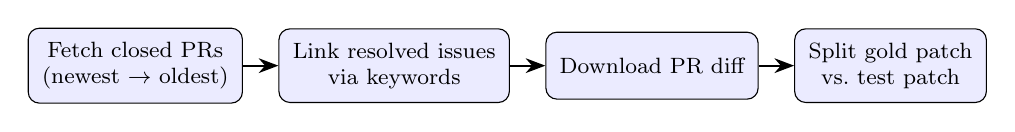
\begin{tikzpicture}[node distance=0.45cm, every node/.style={font=\footnotesize},
    box/.style={draw, rounded corners, fill=blue!8, minimum height=0.85cm, inner sep=5pt, align=center},
    arrow/.style={-{Stealth[length=2.5mm]}, thick}]
    \node[box] (pr) {Fetch closed PRs\\ (newest $\rightarrow$ oldest)};
    \node[box, right=of pr] (link) {Link resolved issues\\ via keywords};
    \node[box, right=of link] (diff) {Download PR diff};
    \node[box, right=of diff] (split) {Split gold patch\\ vs.\ test patch};
    \draw[arrow] (pr) -- (link);
    \draw[arrow] (link) -- (diff);
    \draw[arrow] (diff) -- (split);
\end{tikzpicture}
\end{center}
\begin{itemize}
    \setlength{\itemsep}{5pt}
    \item \textbf{PR fetching}: GitHub API, up to 3{,}000 PRs per repository; automatic rate-limit backoff.
    \item \textbf{Issue linking}: search PR titles, descriptions and commit messages for resolving references such as \textit{fixes \#123} or \textit{closes \#123}.
    \item \textbf{Diff handling}: use \texttt{unidiff} to separate test changes from the production patch.
    \item \textbf{Output}: \stat{4.69M} PRs collected across the \stat{7,773}-repository mining list.
\end{itemize}
\end{frame}

% -----------------------------------------------------------------------------
% Slide 4: Pipeline 3/3 - Task Instance Construction
% -----------------------------------------------------------------------------
\begin{frame}{Data Collection: Building Task Instances}
\begin{center}
\stepstrip{4}{4}
\end{center}
\vspace{0.1cm}
\begin{center}
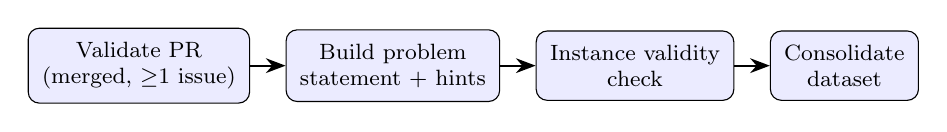
\begin{tikzpicture}[node distance=0.45cm, every node/.style={font=\footnotesize},
    box/.style={draw, rounded corners, fill=blue!8, minimum height=0.85cm, inner sep=5pt, align=center},
    arrow/.style={-{Stealth[length=2.5mm]}, thick}]
    \node[box] (valid) {Validate PR\\ (merged, $\geq$1 issue)};
    \node[box, right=of valid] (ps) {Build problem\\ statement + hints};
    \node[box, right=of ps] (check) {Instance validity\\ check};
    \node[box, right=of check] (out) {Consolidate\\ dataset};
    \draw[arrow] (valid) -- (ps);
    \draw[arrow] (ps) -- (check);
    \draw[arrow] (check) -- (out);
\end{tikzpicture}
\end{center}
\begin{columns}[T]
\begin{column}{0.48\textwidth}
\begin{block}{Instance Fields}
\begin{itemize}
    \setlength{\itemsep}{3pt}
    \item \textbf{Issue text}: linked issue title and body.
    \item \textbf{Optional hints}: issue comments from before the first PR commit.
    \item \textbf{Traceability}: repository, base commit, patches and instance ID.
\end{itemize}
\end{block}
\end{column}
\begin{column}{0.48\textwidth}
\begin{block}{Filters \& Output}
\begin{itemize}
    \setlength{\itemsep}{3pt}
    \item Keep \textbf{merged} PRs with a linked issue, non-empty patch and issue text.
    \item Group by repository, shuffle within each repo and remove test patches.
    \item Output: \stat{396K} issue--patch tasks.
\end{itemize}
\end{block}
\end{column}
\end{columns}
\end{frame}

% -----------------------------------------------------------------------------
% Slide 5: Processing - Function Labels & Negatives (Steps 5-6)
% -----------------------------------------------------------------------------
\begin{frame}{Data Processing: Function Labels \& Negatives}
\begin{center}
\stepstrip{5}{6}
\end{center}
\vspace{0.1cm}
\begin{columns}[T]
\begin{column}{0.48\textwidth}
\begin{block}{Step 5 --- Function-Level Labeling}
\small
\begin{itemize}
    \setlength{\itemsep}{4pt}
    \item Reconstruct the code at the base commit and extract Python functions and methods.
    \item Map patch changes to \textbf{existing functions} to obtain positive (issue, function) examples.
    \item Retain code and source paths for ranking and navigation in the planned app.
\end{itemize}
\end{block}
\end{column}
\begin{column}{0.48\textwidth}
\begin{block}{Step 6 --- Negative Mining \& Filtering}
\small
\begin{itemize}
    \setlength{\itemsep}{4pt}
    \item Score candidate functions with a pretrained code encoder and select challenging negatives from the same repository.
    \item Apply rank-based filtering to positive examples and candidate negatives.
    \item Export issue--function candidate lists for ranking experiments.
\end{itemize}
\end{block}
\end{column}
\end{columns}
\end{frame}

% -----------------------------------------------------------------------------
% Slide 6: Dataset at a Glance
% -----------------------------------------------------------------------------
\begin{frame}{Collected Data Overview}
\small
\begin{columns}[T]
\begin{column}{0.52\textwidth}
\begin{block}{Key Statistics}
\footnotesize
\begin{tabular}{@{}l r@{}}
\toprule
\textbf{Item} & \textbf{Count} \\
\midrule
Initial PyPI packages & \stat{11,000} \\
GitHub repository candidates & \stat{7,773} \\
Pull requests collected & \stat{4.69M} \\
Task instances (issues + patches) & \stat{396K} \\
\bottomrule
\end{tabular}
\end{block}
\end{column}
\begin{column}{0.44\textwidth}
\begin{block}{Instance Schema}
\footnotesize
\texttt{\{\\
\hspace*{0.25cm}"instance\_id": ...,\\
\hspace*{0.25cm}"repo": ...,\\
\hspace*{0.25cm}"base\_commit": ...,\\
\hspace*{0.25cm}"issue\_numbers": [...],\\
\hspace*{0.25cm}"patch": ...,\\
\hspace*{0.25cm}"problem\_statement": ...,\\
\hspace*{0.25cm}"hints\_text": ...,\\
\hspace*{0.25cm}"created\_at": ...\\
\}}
\end{block}
\end{column}
\end{columns}
\end{frame}

% -----------------------------------------------------------------------------
% Slide 6: Distributions & Data Quality
% -----------------------------------------------------------------------------
\begin{frame}{Data Distributions \& Quality}
\small
\begin{columns}[T]
\begin{column}{0.48\textwidth}
\begin{block}{Issue / Problem Statement Length}
\begin{center}
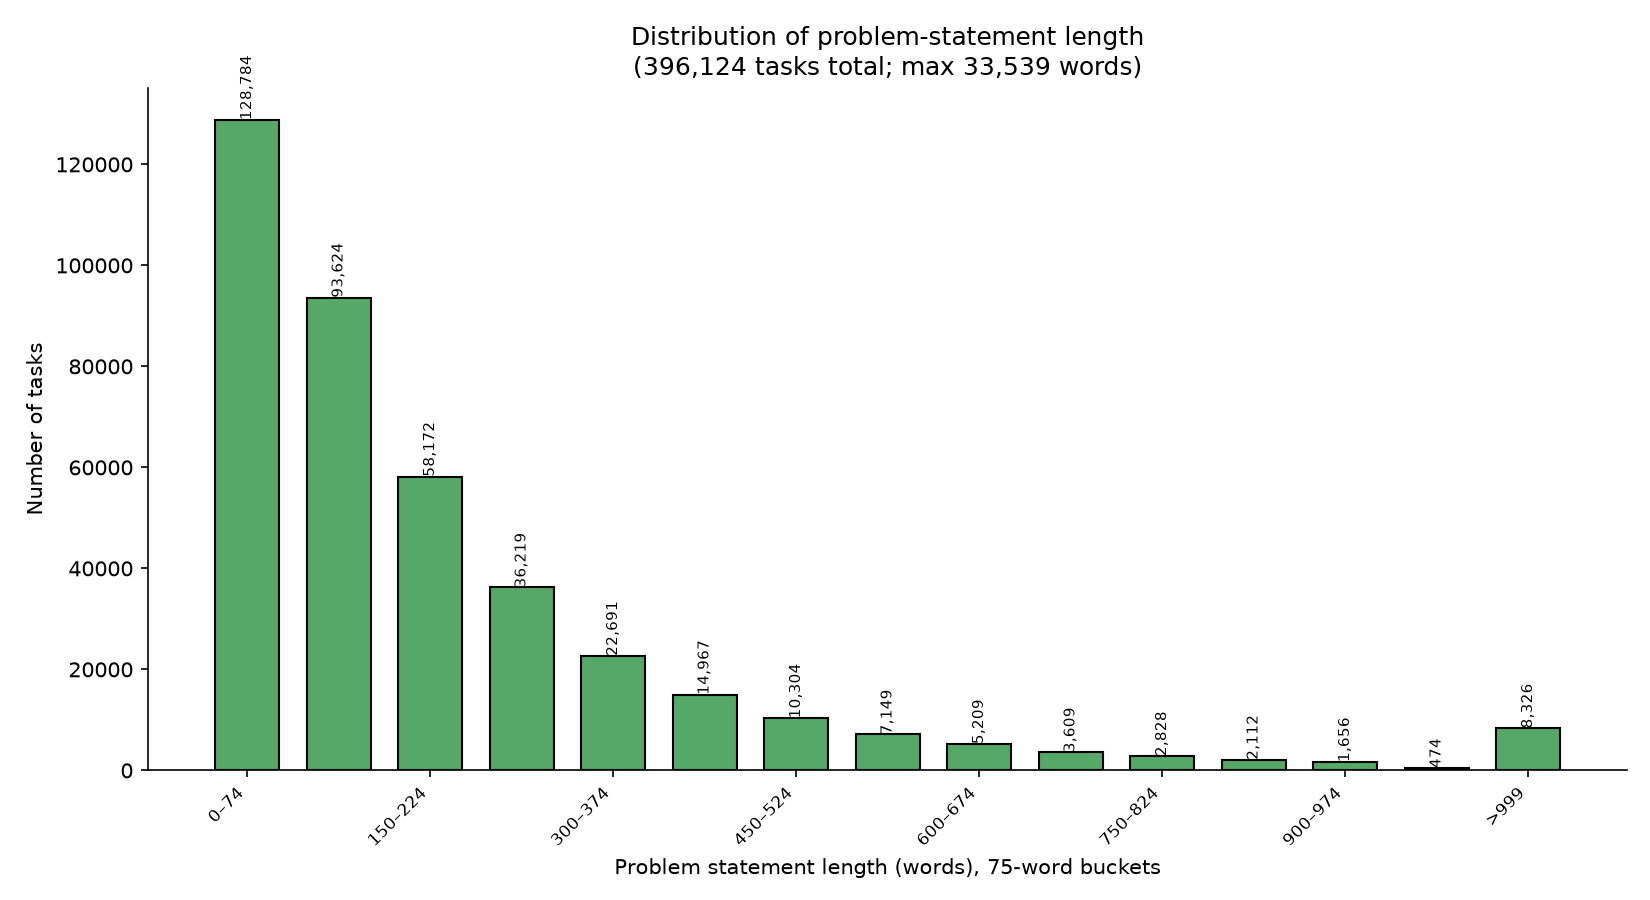
\includegraphics[width=5.6cm]{images/fig5_problem_statement_length_histogram.png}
\end{center}
\end{block}
\end{column}
\begin{column}{0.48\textwidth}
\begin{block}{Patch Breadth (files per task)}
\begin{center}
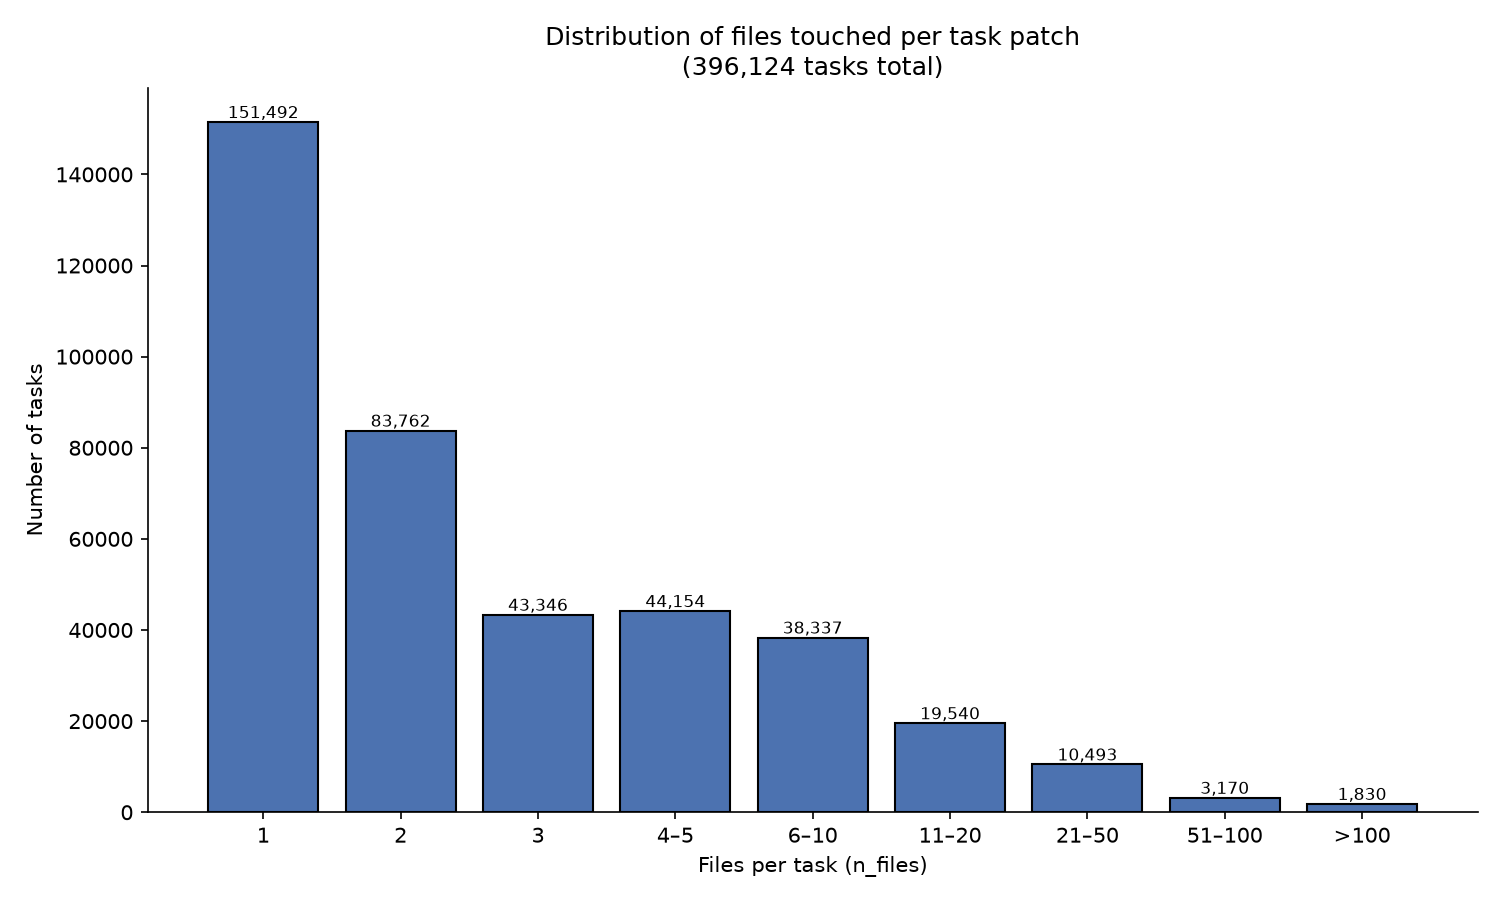
\includegraphics[width=5.6cm]{images/fig2_files_per_task_histogram.png}
\end{center}
\end{block}
\end{column}
\end{columns}
\vspace{0.2cm}
\begin{itemize}
    \setlength{\itemsep}{3pt}
    \item \textbf{Issue length}: about 56\% have fewer than 150 words, motivating analysis of missing context.
    \item \textbf{Patch breadth}: about 59\% touch one or two files, but broader tasks can have multiple targets.
    \item \textbf{Next checks}: audit label relevance and duplicates, and inspect parsing failures.
\end{itemize}
\end{frame}

% -----------------------------------------------------------------------------
% Evaluation of the data science method and the application
% -----------------------------------------------------------------------------
\begin{frame}{Evaluation Plan}
\small
\begin{columns}[T]
\begin{column}{0.48\textwidth}
\begin{block}{Ranking Quality \& Data Analysis}
\begin{itemize}
    \setlength{\itemsep}{5pt}
    \item \textbf{Comparisons}: BM25 keyword search, pretrained code embeddings and optional fine-tuning.
    \item \textbf{Measures}: Recall@5 / Recall@10 for target coverage and MRR for the first relevant result.
    \item \textbf{Data experiments}: compare filtering choices and performance across issue lengths and patch sizes.
    \item \textbf{Validation}: separate repositories across training, validation and test sets.
\end{itemize}
\end{block}
\end{column}
\begin{column}{0.48\textwidth}
\begin{block}{Application Usefulness}
\begin{itemize}
    \setlength{\itemsep}{5pt}
    \item \textbf{Speed}: measure initial indexing time and query response time separately.
    \item \textbf{User task}: compare time to find relevant code with ordinary repository search.
    \item \textbf{Usability}: test issue submission, result inspection and navigation to source code.
    \item \textbf{Feedback}: collect relevance judgments and review failure cases for later improvements.
\end{itemize}
\end{block}
\end{column}
\end{columns}
\end{frame}

% -----------------------------------------------------------------------------
% Progress and application delivery roadmap
% -----------------------------------------------------------------------------
\begin{frame}{Summary \& Next Steps}
\small
\begin{columns}[T]
\begin{column}{0.48\textwidth}
\begin{block}{Current Progress}
\begin{itemize}
    \setlength{\itemsep}{5pt}
    \item Implemented collection and processing scripts for linked issues, patches and function candidates.
    \item Reported collection: \stat{396K} task instances, with \stat{7,773} repository candidates in the mining list.
    \item Initial EDA describes issue lengths and patch breadth. Label auditing and final filtering remain.
\end{itemize}
\end{block}
\end{column}
\begin{column}{0.48\textwidth}
\begin{block}{Next Steps \& Final Deliverable}
\begin{itemize}
    \setlength{\itemsep}{4pt}
    \item \textbf{Data}: finalize filters and labels, including new/deleted functions and addition-only edits.
    \item \textbf{Ranking}: compare baselines and select a method using held-out repositories.
    \item \textbf{Application}: build the indexing service, localization API and web interface. Explore an extension integration.
    \item \textbf{Delivery}: demonstrate issue submission, ranked code results and source navigation, then evaluate with users.
\end{itemize}
\end{block}
\end{column}
\end{columns}
\end{frame}

\setbeamertemplate{background canvas}{}
\useStyleLogoOnly
\hustthankyou

\end{document}
